\documentclass{scrartcl}
\usepackage{listings}
\usepackage{xcolor}
\usepackage{amssymb}
\usepackage[colorlinks=true, urlcolor=blue, linkcolor=red]{hyperref}
\usepackage{graphicx}

\definecolor{lightcyan}{HTML}{E0FFFF}




\begin{document}
    \lstset{
        language=Java,
        %numbers=left,
        stepnumber=1,
        numbersep=5pt,
        backgroundcolor=\color{lightcyan},
        showspaces=false,
        showstringspaces=false,
        showtabs=false,
        tabsize=2,
        captionpos=b,
        breaklines=true,
        breakatwhitespace=true,
        title=\lstname,
        basicstyle=\small
    }

\section{Data Types}

\subsection{Date and Time}

\subsubsection{\lstinline$ LocalDate $}

    LocalDate is an immutable date-time object that represents a date, often viewed as year-month-day. Other date fields, such as day-of-year, day-of-week and week-of-year, can also be accessed.

    \begin{lstlisting}
        // to obtain, e.g.
        static LocalDate of(int year, int month, int dayOfMonth)
        static LocalDate of(int year, Month month, int dayOfMonth)
        static LocalDate ofInstant(Instant instant, ZoneId zone)
        static LocalDate parse(CharSequence text, DateTimeFormatter formatter)

        // instance methods, e.g.
        // return a copy!
        LocalDateTime atTime(int hour, int minute, int second, int nanoOfSecond)
        LocalDateTime atTime(LocalTime time)

        int getDayOfMonth()
        DayOfWeek getDayOfWeek()
        int getDayOfYear()
        Month getMonth()
        int getMonthValue()
        int getYear()

        // same for plus
        // return a copy!
        LocalDate minus(long amountToSubtract, TemporalUnit unit)
        LocalDate minusDays(long daysToSubtract)
        LocalDate minusMonths(long monthsToSubtract) //etc
    \end{lstlisting}

    Beware immutability:
    \begin{lstlisting}
        var date = LocalDate.of(2022, Month.APRIL, 30);
        date.plusDays(2); // does not change date
    \end{lstlisting}

\subsubsection{\lstinline$ LocalTime $}

    LocalTime is an immutable date-time object that represents a time, often viewed as hour-minute-second. Time is represented to nanosecond precision. For example, the value "13:45.30.123456789" can be stored in a LocalTime.

    \begin{lstlisting}
        // to obtain, e.g.
        static LocalTime of(int hour, int minute, int second, int nanoOfSecond)
        static LocalTime ofInstant(Instant instant, ZoneId zone)

        // instance methods, e.g.
        // return a copy!
        LocalDateTime atDate(LocalDate date)

        int getHour()
        int getMinute() //etc.

        // same for minus
        // return a copy!
        LocalTime plus(long amountToAdd, TemporalUnit unit)
        LocalTime plusNanos(long nanosToAdd) // etc.

        // return a copy!
        LocalTime withHour(int hour)
        LocalTime withMinute(int minute) //etc.
        \end{lstlisting}

\subsubsection{\lstinline$ LocalDateTime $}

    \begin{lstlisting}
        // to obtain, e.g.
        static LocalDateTime of(int year, Month month, int dayOfMonth, int hour, int minute, int second, int nanoOfSecond)
        static LocalDateTime of(LocalDate date, LocalTime time)
        // instance methods analogous to above
    \end{lstlisting}

\subsubsection{\lstinline$ Month $}

    In addition to the textual enum name, each month-of-year has an int value (1-12).
    Do not use ordinal() to obtain the numeric representation of Month. Use getValue() instead.

    \begin{lstlisting}
        // to obtain, e.g.
        static Month of(int month)
        Month e = Month.of(10); // DECEMBER
        static Month valueOf(String name)
        Month m = Month.valueOf("DECEMBER"); // DECEMBER

        // instance methods, e.g.
        int getValue()
        int length(boolean leapYear)
        minus(long months)
        plus(long months)
    \end{lstlisting}

\subsubsection{\lstinline$ ChronoUnit $}

    \begin{lstlisting}

        // to obtain, e.g.
        static ChronoUnit valueOf(String name)

        // instance methods, e.g.
        <R extends Temporal> R addTo(R temporal, long amount) // returns a copy!
        long between(Temporal temporal1Inclusive, Temporal temporal2Exclusive)

        // Usage example
        // https://stackoverflow.com/questions/77587361/chronounit-months-inconsistency-between-addto-and-between
        var d1 = OffsetDateTime.parse("2023-01-31T10:00:00Z");
        var d2 = ChronoUnit.MONTHS.addTo(d1, 1);
        d2 = ChronoUnit.HOURS.addTo(d2, 23);
        System.out.println(ChronoUnit.MONTHS.between(d1, d2)); // 0
        }
\end{lstlisting}

\subsubsection{\lstinline$ Instant $}

     An \lstinline$ Instant $ represents a specific moment in time using GMT.
    Consequently, there is no time zone information.

    \begin{lstlisting}
        // to obtain, e.g.
        static Instant from(TemporalAccessor temporal)
        static Instant now()
        static Instant ofEpochMilli(long epochMilli)

        // instance methods, e.g.
        OffsetDateTime atOffset(ZoneOffset offset)
        ZonedDateTime atZone(ZoneId zone)

        Instant minus(long amountToSubtract, TemporalUnit unit) //returns copy! others too
        Instant minus(TemporalAmount amountToSubtract)

        Instant minusMillis(long millisToSubtract)
        Instant minusNanos(long nanosToSubtract)

        var instant = trainDay.toInstant(); // will not compile if this is a LocalDateTime!

    \end{lstlisting}

\subsubsection{\lstinline$ Period $}

    This class models a quantity or amount of time in terms of years, months and days. See Duration for the time-based equivalent to this class.

    Durations and periods differ in their treatment of daylight savings time when added to ZonedDateTime. A Duration will add an exact number of seconds, thus a duration of one day is always exactly 24 hours. By contrast, a Period will add a conceptual day, trying to maintain the local time.

    For example, consider adding a period of one day and a duration of one day to 18:00 on the evening before a daylight savings gap. The Period will add the conceptual day and result in a ZonedDateTime at 18:00 the following day. By contrast, the Duration will add exactly 24 hours, resulting in a ZonedDateTime at 19:00 the following day (assuming a one hour DST gap).

    The supported units of a period are YEARS, MONTHS and DAYS. All three fields are always present, but may be set to zero.

    The period is modeled as a directed amount of time, meaning that individual parts of the period may be negative.

    \begin{lstlisting}
        // to obtain, e.g.
        static Period between(LocalDate startDateInclusive, LocalDate endDateExclusive)
        static Period of(int years, int months, int days)
        static Period ofDays(int days) // other fields will be 0
        static Period ofMonths(int months)

        // instance methods, e.g.
        Temporal addTo(Temporal temporal)
        Period minusDays(long daysToSubtract) // all return copies!
        minusMonths(long monthsToSubtract)

        Period withMonths(int months) // copies, too!
        Period withYears(int years)

        int getDays()
        \end{lstlisting}

 \subsubsection{\lstinline$ Duration $}

    This class models a quantity or amount of time in terms of seconds and nanoseconds. It can be accessed using other duration-based units, such as minutes and hours. In addition, the DAYS unit can be used and is treated as exactly equal to 24 hours, thus ignoring daylight savings effects.

    See Period for the date-based equivalent to this class.

     \begin{lstlisting}
     // to obtain, e.g.
     static Duration of(long amount, TemporalUnit unit)
     // convenience method
     static Duration ofDays(long days)

     // instance methods, e.g.
     Duration dividedBy(long divisor) // all these copy
     long dividedBy(Duration divisor)

     long get(TemporalUnit unit)
     int getNano()
     long getSeconds()

     // static methods, e.g.
     // throws UnsupportedTemporalTypeException if passed a LocalDate
     Duration between(LocalDateTime now, LocalDateTime other);
     \end{lstlisting}

 \subsection{String and StringBuilder}
 \subsubsection{\lstinline$ String $}

    \begin{lstlisting}

      // Instance methods e.g.
     char charAt(itn index)
     boolean contains(CharSequence s);
     String concat(String str);
     int indexOf(int ch);
     String replace(char oldChar, char newChar);
     String[] split(String regex);

     // strip()-related methods (these are the only ones)
     strip(), stripLeading(), stripTrailing(), stripIndent()

     // indent():
     // indent(n) splits into lines and then indents each; also adds newline after the last line if there's none.
     // indent(0) does not change the indentation, but still adds a newline after the last line
     // indent(-n) removes indentation iff there is any, and also adds a newline after the last line

     // indent() example
     var phrase = "prickly \nporcupine";
     System.out.println(phrase);
     System.out.println(".........................................");
     System.out.println(phrase.indent(1));
     System.out.println(".........................................");
     System.out.println(phrase.indent(0));
     System.out.println(".........................................");
     System.out.println(phrase.indent(-1));
     System.out.println(".........................................");

     // Output:
     prickly
     porcupine
     .........................................
      prickly
      porcupine

     .........................................
     prickly
     porcupine

     .........................................
     prickly
     porcupine

     .........................................


     // translateEscapes()
     // these print 2 lines:
     System.out.println("cheetah\ncub");
     System.out.println("cheetah\ncub".translateEscapes());
     System.out.println("cheetah\\ncub".translateEscapes());
     - this prints 1:
     System.out.println("cheetah\\ncub");

     // there is no reverse()
     \end{lstlisting}

     Strings use lexicographic ordering (based on the Unicode representation) for \lstinline|compareTo()|.

     In lexicographic ordering, if two strings are different, then either they have different characters at some index that is a valid index for both strings, or their lengths are different, or both.

     If they have different characters at one or more index positions, let k be the smallest such index; then the string whose character at position k has the smaller value, as determined by using the < operator, lexicographically precedes the other string. In this case, compareTo returns the difference of the two character values at position k in the two string - that is, the value:

     \begin{lstlisting}

         this.charAt(k)-anotherString.charAt(k);

     \end{lstlisting}

     \textit{If there is no index position at which they differ, then the shorter string lexicographically precedes the longer string.} In this case, compareTo returns the difference of the lengths of the strings - that is, the value:

     \begin{lstlisting}

        this.length()-anotherString.length();

     \end{lstlisting}




 \subsubsection{\lstinline$ StringBuilder $}

    \begin{lstlisting}

        // instance methods, e.g.

        // Appends a subsequence of the specified CharSequence to this sequence
        // so: start and end refer to the new sequence!
        // If s is null, then this method appends characters as if the s parameter was a sequence containing the four characters "null".
        StringBuilder append(CharSequence s, int start, int end) throws IndexOutOfBoundsException

        // inserts a subsequence of the specified CharSequence into this sequence.
        // dstOffset is the offset in this sequence.
        StringBuilder insert(int dstOffset, CharSequence s, int start, int end) throws IndexOutOfBoundsException

        //  Replaces the characters in a substring of this sequence with characters in the specified String.
        StringBuilder replace(int start, int end, String str) throws StringIndexOutOfBoundsException


        StringBuilder delete(int start, int end)

        // beware: returns a new String!
        String substring(start, end) throws StringIndexOutOfBoundsException

        char charAt(int index)

        IntStream chars()

        int indexOf(String str)

        int length()


    \end{lstlisting}

\subsection{Numbers}
\subsubsection{Number types: automatic promotion}

    Integer literals are considered int by default (size notwithstanding). But they can be automatically promoted to long, float, or double.

    \begin{lstlisting}
        final ___ song = 6; // can be int, long, float, double (automatic promotion from int)
    \end{lstlisting}

    When used as an argument to overloaded methods, ints will preferentially be promoted to long (or double) before autoboxing to Integer is considered.

\subsubsection{Autoboxing}

    Beware: cannot autobox and promote at the same time!

    \begin{lstlisting}

    \end{lstlisting}


\subsubsection{Math methods}
    \begin{lstlisting}
        Math.round() // double -> double
        Math.max() // overloaded, returns passed-in type
        Math.pow() // double -> double
    \end{lstlisting}

\subsubsection{Parsing Strings}
    \begin{lstlisting}
        var numPigeons = Long.parseLong("100"); // returns long
        var numPigeons2 = Long.valueOf("100"); // returns Long
    \end{lstlisting}

    Examples:
    \begin{lstlisting}
        // compiles - Boolean's being lenient
        Boolean.valueOf("8").booleanValue() // false

        // Character has no byteValue()
        Character.valueOf('x').byteValue(); // does not compile

        // cannot have underscore next to decimal point
        Double.valueOf("9_.3").byteValue(); // NumberFormatException

        Long.valueOf(128).byteValue(); // - 128
    \end{lstlisting}

\subsection{Arrays}

    These are all legal array declarations:

    \begin{lstlisting}
        // no var allowed
        String[][] gamma;
        String[] delta[];
        String epsilon[][];
    \end{lstlisting}

\subsection{\lstinline|java.util.Optional<T>|}

\begin{lstlisting}

   // to obtain:
   static <T> Optional<T> 	empty()
   static <T> Optional<T> 	of(T value)empty Optional
   // if value null return
   static <T> Optional<T> 	ofNullable(T value)

   // instance methods, e.g.

   // If a value is present and predicate matched, return Optional with value, otherwise return an empty Optional.
   Optional<T> 	filter(Predicate<? super T> predicate)

   // may throw NoSuchElementException
   T get()

   void ifPresent(Consumer<? super T> consumer)

   // If value present, apply mapping function to it, and if the result is non-null, return an Optional describing the result.
   <U> Optional<U> 	map(Function<? super T,? extends U> mapper)

   // Return the value if present, otherwise return other.
   T orElse(T other)

   //  Return value if present, otherwise invoke other
   T orElseGet(Supplier<? extends T> other)

   <X extends Throwable> T orElseThrow(Supplier<? extends X> exceptionSupplier)

\end{lstlisting}



\section{Operators}
\subsection{Kinds}
\subsubsection{Logical Operators}
    \begin{lstlisting}
        &&
        ||
        // no ~!
    \end{lstlisting}

\subsubsection{Bitwise Operators: Logical}
    \begin{lstlisting}
        &
        int result = 5 & 6; // 4    101 & 110 = 100
        |
        int result = 5 | 6; // 7    101 | 110 = 111
        ^
        int result = 5 ^ 6; // 3    101 ^ 110 = 011
        ~
        int result = ~6; // -7      0000 0110 -> 1111 1001 -> 0000 0110 + 1 -> 0000 0111
    \end{lstlisting}

    \subsubsection{Bitwise NOT, complements, etc.}

    Ex. 1: Bitwise NOT computation steps:

    \begin{enumerate}
        \item to compute ~6, first write 6 in binary: 0000 0110
        \item negate each bit: 1111 1001 // this is the 1's complement
        \item to get the 2's complement (since numbers are stored as 2’s complement), add 1: 1111 1010
    \end{enumerate}

    Ex. 2: To find the binary representation of -17, take the 2's complement of 17:

    \begin{enumerate}
        \item 17 = 0001 0001
        \item Take the bitwise complement: 1110 1110
        \item Add 1: 1110 1110 + 1 = 1110 1111
    \end{enumerate}

    Ex. 3: Take the 2's complement of negative number:
    \begin{enumerate}
        \item Start from binary -17: 1110 1111
        \item     Take the the bitwise complement: 0001 0000
        \item     Add 1: 0001 0001
        \item     This gets back the 17!
    \end{enumerate}

    Ex. 4: To find the decimal representation of a number given in binary, reverse steps
   \begin{enumerate}
       \item  Subtract 1: 1110 1111 - 1 = 1110 1110
       \item     Take the complement of the complement: 0001 0001
       \item     Change from base 2 back to base 10 16 + 1 = 17
       \item     Rewrite this as a negative integer: -17
   \end{enumerate}

\subsubsection{Bitwise operators: arithmetic}
    \begin{lstlisting}

        // shift left (signed)
        12  << 2: 48 // *2^n

        // shift right (signed)
        12 >> 2: 3 // 1100 -> 0011 (pos.: fill with 0)
        -12 >> 2: -3 // (neg..: fill with 1)

        // shift right (unsigned)
        12 >>> 2: 3 // 1100 -> 0011
        -12 >>> 2: 1073741821 // fill with 0 too
    \end{lstlisting}

\subsection{Precedence}

    Default evaluation order is left-to-right.

    \begin{tabular}{|l|c|r|}
        \hline
        Post-­unary operator& x++, x-- &  \\
        \hline
        Pre-­unary operator& ++x, ++x &  \\
        \hline
        Other unary operators& -­, !,$\sim$, + &  Right-­to-­left \\
        \hline
        Cast(type)reference&  &  Right-­to-­left \\
        \hline
        Multiplication/division/modulus& *, /, \% &  \\
        \hline
        Addition/subtraction& +, - &  \\
        \hline
        Shift operators& $\ll, \gg, \ggg$ &  \\
        \hline
        Relational operators & $<$, $>$, $<=$, $>=$, instanceof & \\
        \hline
        Equal to/not equal to& ==, != &\\
        \hline
        Logical AND& \& &  \\
        \hline
        Logical exclusive OR& \textasciicircum \\
        \hline
        Logical inclusive OR& $|$ &  \\
        \hline
        Conditional OR& $||$ &  \\
        \hline
        Conditional AND& \&\& &  \\
        \hline
        Ternary operator& e1 ? e2 : e3 & Right-­to-­left\\
        \hline
        Assignment operators& =, +=, -­=, *=, /=, \%=, \&=, \textasciicircum, & Right-­to-­left\\
        & $|$, $<<=$ , $>>=$, $>>>=$ & \\
        \hline
        Arrow operator& $->$ &  \\\\
        \hline
    \end{tabular}
     \\

    In a nutshell:

    \begin{itemize}
        \item shift ops after +, -
        \item relational before equality before logical
        \item \& $|$ before \&\& $||$
        \item ternary thereafter but before assignment
        \item assignment last
    \end{itemize}

\section{Syntax}
\subsection{Allowed variable names}

    Names may contain: underscore, currency symbol, numbers, letters (first may not be a number)

\subsection{Reserved Words}

    See \ref{fig:reserved-words}.

    \begin{figure}
        \centering
        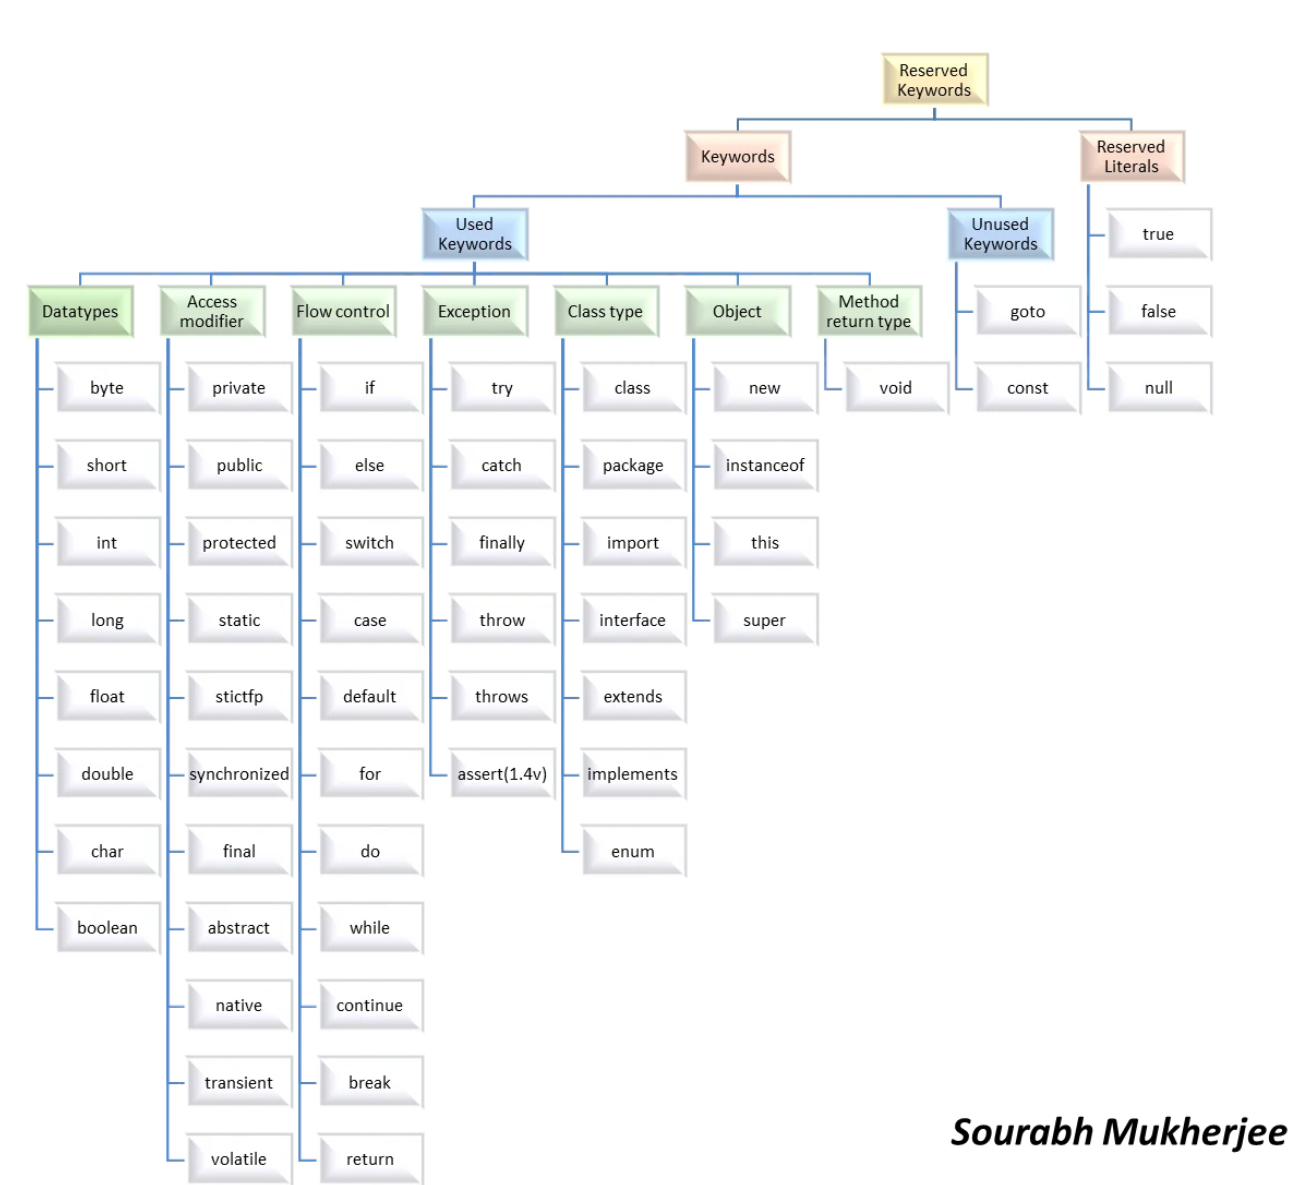
\includegraphics[width=1\linewidth]{reserved-words}
        \caption{Reserved Words}
        \label{fig:reserved-words}
    \end{figure}

\subsection{Variable declarations and initialization topics}

    For instance variables, on a single line only one type should be specified.



\subsection{Text blocks}

    Imagine a vertical line drawn on the leftmost non-­whitespace character in the text block. Everything to the left of it is incidental whitespace, and everything to the right is essential whitespace.

    Note:
    \begin{itemize}
        \item  \textbackslash at end of line means the line gets continued
        \item Space at end of line is ignored
        \item \textbackslash s yields two spaces
        \item  \textbackslash n yields additional line break
    \end{itemize}

    Example:

    \begin{lstlisting}
        // starting quotes on sep. line
        String block = """
        doe \
         // ending quotes on same line
        doof""";

         var quotes = """
        \"The Quotes that Could\" // could remove both backslashes here
        \"\"\"                    // could remove 2 backslashes (otherwise end of format string)
        """;
    \end{lstlisting}

\subsection{var}

    A var cannot be initialized with a null value without giving a type.

    var cannot be used in a multiple-­variable assignment.

\subsection{underscore}

    An underscore can be placed in any numeric literal, as long as it is not at the beginning, at the end, or next to a decimal point. Underscores can even be placed next to each other.

\subsection{switch}

\subsubsection{General}

        \begin{itemize}
            \item Supports the following data types as arguments to switch(): enum, byte, Byte, short, Short, char, Character, int, Integer,
            String, var (if resolves to one of those types)
            \item Does not support: boolean, Boolean, double, Double, float, Float, long, Long
         \end{itemize}

\subsubsection{Statement}

    \begin{itemize}
        \item The value passed to a \textit{case} (not switch!) statement must be a constant, a literal value, or a final variable (not, e.g., \lstinline$ case red:  $)
        \item May use comma to separate case constants in statements: e.g.,
            \begin{lstlisting}
                public int getAverageTemperate(Season s) {
                    switch (s) {
                        default:
                        case WINTER, SUMMER: return 30;
                }}
            \end{lstlisting}
    \end{itemize}

\subsubsection{Expression}

    \begin{itemize}
        \item A switch expression requires all possible case values to be handled, or a default to be added.
        \item switch expressions execute exactly one branch and do not use break statements.
        \item switch expressions need a semicolon.
        \item Can omit default clause in when either all the values of an enum are covered or no value is returned.
        \item Case labels must be compile-time constants.
        \item Every path must return a value.
    \end{itemize}

    Example:

    \begin{lstlisting}
        case 10 -> {"Jane";} // yield implied
        case 20 -> {yield "Lisa";}
        // expression may also have multiple values passed to case
        case 30, 40 -> "Kelly";
        default -> "Unassigned";
    \end{lstlisting}

\subsection{ for (x : y)}

     A for-­each loop accepts arrays and classes that implement java.lang.Iterable, such as List. Not: String, StringBuilder

\subsection{Flow Scoping}

    Example:

    \begin{lstlisting}
        static void printIfString(Object o) {
            if (!(o instanceof String s)) {
                // 's' is NOT in scope
                return;
            } else {
                // 's' is in scope
                // s is a string
                System.out.println(s);
            }
        }

        // this is valid:
        if (x instanceof Foo(var v) && v != null) {
            A;
        }

        //this is NOT:
        if (x instanceof Foo(var v) || v != null) {
            A;
        }
    \end{lstlisting}

    \begin{lstlisting}
        if (number instanceof Integer i && Math.abs(i) == 0) // ok
        if (number instanceof Integer i || Math.abs(i) == 0) // i not defined
        if (number instanceof int i && Math.abs(i) == 0) // can't use primitives
    \end{lstlisting}

\subsection{Loops}

    for and while (but not do-while) don't need braces if just one statement follows.

    \begin{lstlisting}
        while (i<6) System.out.println("");
        for (;;) System.out.println();
    \end{lstlisting}

\section{Methods and functions}
\subsection{General notes}

    Java does not support setting default method parameter values.

\subsection{Pass-by-value and references}

    Java creates a copy of references and pass it to the invoked method,     but they still point to same memory reference. Thus, changes made to the object are reflected in the caller.

    \textit{However}, changes are not reflected back if we \textit{change the reference itself} to refer some other location or object!


\subsection{Method references}

    \subsubsection{static methods}

    \begin{lstlisting}
        interface Converter {
            long round(double num);
        }

        Converter methodRef = Math::round;

        // same as lambda
        Converter lambda = x -> Math.round(x);
    \end{lstlisting}

    Like with lambdas, Java uses type inference to infer that x here is a double.

    \subsubsection{Instance methods on an instance object}

    Here are two ways of calling an \textit{instance method that takes no parameters}.

    With the first, the interface method, too, takes no parameters:


    \begin{lstlisting}
        interface StringChecker {
            boolean check();
        }

        var str = "";
        // uses concrete instance, not class method
        StringChecker methodRef = str::isEmpty;

        // same as lambda
        StringChecker lambda = () -> str.isEmpty();
    \end{lstlisting}

    With the second, the interface method takes one parameter:

    \begin{lstlisting}
        interface StringParameterChecker {
            boolean check(String text);
        }

        // now uses class!
        StringParameterChecker methodRef = String::isEmpty;

        // same as lambda
        StringParameterChecker lambda = s -> s.isEmpty();
    \end{lstlisting}

    How about \textit{instance methods that take one or more parameters}?
    Here, the \textit{interface method takes two parameters}:

        \begin{lstlisting}
            // the lambda
            StringTwoParameterChecker lambda = (s, p) -> s.startsWith(p);

            interface StringTwoParameterChecker {
                boolean check(String text, String prefix);
            }

            // uses class method!
            StringTwoParameterChecker methodRef = String::startsWith;

            // first parameter is instance, all others are method parameters
            methodRef.check("Zoo", "A"));
        \end{lstlisting}

    \subsubsection{Constructors}

    This example mimics a \textit{lambda calling a constructor that takes no parameters}.

    \begin{lstlisting}
        interface EmptyStringCreator {
            String create();
        }

        EmptyStringCreator methodRef = String::new;
        var myString = methodRef.create();
        System.out.println(myString.equals("Snake"))

        // lambda
        EmptyStringCreator lambda = () -> new String();

    \end{lstlisting}

    Here, Java sees that we are passing a String parameter and \textit{calls the constructor of String that takes such a parameter}:

    \begin{lstlisting}

        // lambda
        StringCopier lambda = x - new String(x);

        interface StringCopier {
            String copy(String value);
        }

        // same method reference!
        StringCopier methodRef = String::new;

        var myString = methodRef.copy("Zebra");

    \end{lstlisting}

\subsection{Mixed notes on functions}
\subsubsection{compose()}

    The \lstinline{a.compose(b)} method calls the Function parameter b before the reference Function variable a.

    To memorize:

    \begin{lstlisting}
        after.compose(before)

        // is like
        after o before

    \end{lstlisting}


\section{Classes, Interfaces, Records and Enums}
\subsection{General Notes}

\subsubsection{Member (Class and Instance) Variables}

All member fields (static and non-static) are initialized to their default values.

Objects are initialized to null, numeric types to 0 (or 0.0), and boolean to false.

If a static variable is final, it must be initialized, either in the declaration or in a static initializer.

\subsubsection{Inheritance}

    When a parent defines a with-argument constructor only, the child must call the parent constructor explicitly. It is not enough for both to take the same arguments. See:

    \begin{lstlisting}
        class Cinema {
            private String name = "Sequel";
            public Cinema(String name) {
                this.name = name;
            }
        }
        public class Movie extends Cinema {
            private String name = "adaptation";
            public Movie(String movie) {
                this.name = "Remake";
            }
        }
    \end{lstlisting}

    An instance variable with same name in the child hides the parent variable.

    When a parent method is static, the child cannot "override" (\textit{nor complement}) this by a same-arg instance method.

\subsection{Classes}

\subsubsection{Top-level classes}

Top-level classes may only have public or
package access.

\subsubsection{Nested Classes}

    There are four types of nested classes: inner, static, local, and anonymous.
    Nested classes can be public.

    An \textit{inner} class requires an instance of the outer class to use.
    Three ways that are legal:

    \begin{lstlisting}
    public class Dinosaur {
        class Pterodactyl extends Dinosaur {}

        // it all happens in an instance method
        public void roar() {
            var dino = new Dinosaur();

            // uses instance to create inner
            dino.new Pterodactyl();

            // relies on the fact that roar() is an instance method
            //, which means there's an implicit instance of the outer class Dinosaur available
            new Dinosaur.Pterodactyl();

            // The Dinosaur. prefix is optional, though
            new Pterodactyl();
        } }
    \end{lstlisting}

    While a \textit{static} nested class does not:

    \begin{lstlisting}
        new Lion.Den()
    \end{lstlisting}

    A \textit{local} class is commonly defined within a method or block.
    Local classes can only access local variables that are final or effectively final.

    \textit{Anonymous} classes are a special type of local class that does not have a name.
    Anonymous classes are required to extend exactly one class or implement one interface.

    Note:

    \textit{Inner, local, and anonymous} classes can \textit{access private members} of the class in which they are defined, provided the latter two are used inside an instance method.

    \textit{Static} nested classes cannot access the instance variables or methods of the outer class.

    \textit{All four} types of nested classes can now define static variables and methods.

\subsubsection{Sealed Classes}

    A sealed class is a class that restricts which other classes may directly extend it:

    \begin{lstlisting}
         sealed class Friendly extends Mandrill permits Silly {}
    \end{lstlisting}


    Every class that directly extends a sealed class must specify exactly one of the following three modifiers: final, sealed, or non-­sealed.

    Rules regarding \textit{permit}:

    \begin{itemize}
        \item A sealed class/interface must have a permits clause. An exception is that if all the direct subclasses/subinterfaces are defined in the same compilation unit, then the permits clause is not needed.
        \item Beware though: the extends clause still is! See:

\begin{lstlisting}
    // MyClass.java:25: error: cannot find symbol
    //sealed class Friendly extends Mandrill permits Silly {}
    //                  ^
    // symbol: class Mandrill
    // MyClass.java:25: error: invalid permits clause
    //
    sealed class Friendly extends Mandrill permits Silly {}
    //                ^
    // (subclass Silly must extend sealed class)
    // 2 errors
\end{lstlisting}
        \item  If a sealed class C is associated with a \textit{named module}, then every class specified in the permits clause must be associated with the same \textit{module} as C.
        \item If a sealed class C is associated with an \textit{unnamed module} , then every class specified in the permits clause must belong to the same \textit{package} as C.
    \end{itemize}

    Note:

    \begin{itemize}
        \item Sealed classes cannot be final (otherwise the permits clause would make no sense).
        \item   We can have sealed interfaces (permitting both extensions and implementations). There are no sealed enums or records, though.
        Records are implicitly final, so it doesn't make sense to mark them as sealed.
        Enums are either implicitly final (if its declaration contains no enum constants that have a class body) or implicitly sealed (if its declaration contains at least one enum constant that has a class body, in which case the anonymous classes implicitly declared by the enum constants are its only permitted subclasses).
        However, enums (as well as records) may implement a sealed interface:

        \begin{lstlisting}
            sealed interface I permits X, R{ }
            enum X implements I{ }
            record R(int value) implements I{ }
        \end{lstlisting}
        \item While a sealed class is commonly extended by a subclass marked final, it can also be extended by a sealed or non-­sealed subclass marked abstract.
    \end{itemize}

\subsubsection{Final and Immutable Classes}

    - Classes marked as final can’t be extended.
    - Immutable classes do not include setter methods. They must be marked final \textit{or} contain only private constructors.

\subsection{Interfaces}
\begin{itemize}

    \item     \textit{Variables} are always public, static, final. No other modifiers are allowed.

    \item     \textit{Methods} can be either \textit{default} (these are always public), static (always public, must have a body), private, or private and static. Methods cannot be final nor protected. If there is no modifier, a method is implicitly public.

    \item Methods \textit{with a body} must be declared \textit{default, static or private}.

    \item     \textit{Default} methods are implicitly public. There is no modifier that can prevent a default method from being overridden in a class implementing an interface.

    \item Interfaces cannot have a constructor.

    \item     If implementing two interfaces that define a default method with the same signature, classes (incl. abstract classes) have to override it explicitly, or their declaration will not compile. (I.e., this fails on compilation already, not on call. See example.)

    They can then access the inherited ones by calling Interface.super.method() - provided this happens in an instance method, since otherwise super() is not available.

    \begin{lstlisting}
        public class App {
            interface Building {
                default Double getHeight() {
                    return 1.0;
                }
            }
            interface Office {
                public default String getHeight() {
                    return null;
            }
            // does not compile
            abstract class Tower implements Building, Office {}

    \end{lstlisting}

    \item     \textit{Private} methods must contain a body.

    \item     \textit{Static} methods are only accessible with a qualifier. A static method can be invoked from other static or from default method. A static method cannot be overridden or changed in the implementation class. The static methods are implicitly public — there's no need to specify the public modifier.

    \item     Interfaces may contain member type declarations (nested type). A member type declaration in an interface is implicitly static and public. It is permitted to redundantly specify either or both of these modifiers.

    \item Interfaces may contain nested sealed classes or interfaces. No permits clause is necessary, but the sealed class or interface must be followed by an inheriting/extending subclass/interface.


\end{itemize}
\subsection{Records}

    Minimal example:

    \begin{lstlisting}
        // parentheses are required
        public record Crane(int numberEggs, String name) { }
    \end{lstlisting}

    Records may optionally have constructors.

\subsubsection{Record Constructors}

Constructors can be compact or long, as well as canonical or non-canonical.

\paragraph{Canonical or Non-canonical}

Canonical constructors are passed all of the fields mentioned in the record declaration.
Non-canonical constructors may take less (no, even) or more arguments.

\paragraph{Long vs. Compact}

Both the long as well as the short constructor are \textit{canonical constructors}, i.e., they operate on the exact record fields mentioned in the record declaration.

The following is a short constructor. Of those, a record can have at most one (since a short contructor uses the fields specified in the record declaration).

At the end of the compact record constructor, the compiler adds code that sets all the fields to the values passed in the constructor. E.g., if the constructor changes a passed value, the updated value will be given to respective field.

    \begin{lstlisting}
        public Crane { // no parens
            if (numberEggs < 0) throw new IllegalArgumentException();
            // could not be this.name in the compact constructor
            name = name.toUpperCase();
            // long form is automatically called here
        }
    \end{lstlisting}

And this is long constructor (there may be several):

    \begin{lstlisting}
        public Crane(int numberEggs, String name) {
            if (numberEggs < 0) throw new IllegalArgumentException();
            this.numberEggs = numberEggs;
            this.name = name;
        }
    \end{lstlisting}

Constructors may be overloaded:

    \begin{lstlisting}
        public record Crane(int numberEggs, String name) {
            public Crane(String firstName, String lastName) {
                // must be first call, must either call 1) another long constructor or 2) the short or 3) the default constructor
                this(0, firstName + " " + lastName);
        }}
    \end{lstlisting}

    An example where both are present:

    \begin{lstlisting}
        public record Disco(int beats) {
            public Disco(String beats) {
                this(20);
            }
            public Disco {
                beats = 10;
            }
            public int getBeats() {
                return beats;
            }
            public static void main(String[] args) {
                // beats() is provided by default
                // calls default constructor
                System.out.print(new Disco(30).beats());
            }
        }
    \end{lstlisting}


    \paragraph{Records may:}

    \begin{itemize}
    \item implement interfaces:
    \begin{lstlisting}
    public record Crane(int numberEggs, String name) implements Bird {}
    \end{lstlisting}
    \item override a method:
    \begin{lstlisting}
    public record BeardedDragon(boolean fun) {
        // overriding generated accessor
        @Override public boolean fun() { return false; }
        }
    \end{lstlisting}
    \item have any access modifier.
    \item contain nested classes, interfaces, annotations, enums, and other records.
    \item contain instance \textit{methods}.
    \item contain \textit{static} fields, initializers and methods.
    \end{itemize}

    \paragraph{Records may not:}

    \begin{itemize}
        \item extend other classes.
        \item be subclassed, since they are implicitly final.
        \item  declare instance \textit{variables} or instance \textit{initializers}.
    \end{itemize}

\subsection{Enums}

    Like records, enums are implicitly final, and may not be extended, since just as every Record inherits from Record every enum inherits from enum.

    Enums can have constructors, methods, and fields. Methods may be abstract, while the enums themselves may not.

    Enum constants must be declared before everything else.

    Example:

    \begin{lstlisting}
        enum Flavors {
            VANILLA, CHOCOLATE, STRAWBERRY;
            static final Flavors DEFAULT = STRAWBERRY;
        }
    \end{lstlisting}

    Constructors are optional; if provided they are implicitly private. It is ok not to provide any access modifier; public and protected are explicitly disallowed.

    Instance fields may never be of type var. (Only method-local variables may be.)

     \begin{lstlisting}
        enum Animals {
            // When an enum contains any other members, such as a constructor or variable, a semicolon is required:
            MAMMAL(true), INVERTEBRATE(Boolean.FALSE), BIRD(false),REPTILE(false),
            AMPHIBIAN(false),
            // fish is actually an anonymous subclass overriding swim()
            FISH(false) {public int swim() { return 4; }};

            final boolean hasHair;

            // implicitly private
            Animals(boolean hasHair) {this.hasHair = hasHair;}

            public boolean hasHair() { return hasHair; }
            public int swim() { return 0; }
        }

    \end{lstlisting}

    An Enum constructor can accept multiple values. Example:

    \begin{lstlisting}
       public enum Element {
           H("Hydrogen", 1, 1.008f),
           HE("Helium", 2, 4.0026f),
           // ...
           NE("Neon", 10, 20.180f);

           private Element(String label, int atomicNumber, float atomicWeight) {
               this.label = label;
               //
           }
      }


    \end{lstlisting}

    Methods:

    \begin{lstlisting}
        // to obtain:
        static <T extends Enum<T>> T valueOf(Class<T> enumClass, String name)

        // instance method to get the ordinal (starts with 0)
        final int ordinal()

        // returns enum constant; may be overridden
        toString()

        // to iterate over enum constants, the compiler provides values() that returns an array of values in the order they have been defined
        for (var c : Card.values()) /...

    \end{lstlisting}

    Enums implement Comparable; they are sorted in the order they are defined.

\subsection{Overriding, overloading and Hiding}
\subsubsection{Overloading}

    Overloading works also for pairs of primitive + wrapper, e.g.

    \begin{lstlisting}

        public static void main(String... args) {
            System.out.println(new App().woof(5)); // 1
            System.out.println(new App().woof(Integer.valueOf(5))); // 2
        }
        public String woof(int bark) {
            return "1";
        }
        public String woof(Integer bark) {
            return "2";
        }
    \end{lstlisting}

\subsubsection{Overriding and Hiding}

   Methods and variables are considered separately.

    \begin{itemize}
        \item \textit{Variables}

        Instance variables are never overridden. They are always determined by the reference type.

        The same goes for class variables. In the following example,the child class variable hides the parent's class variable; it is thus not a problem that the parent variable is final.

        \begin{lstlisting}

         class A{
             final int fi = 10;
         }
         public class B extends A{
             int fi = 15;
         }
         \end{lstlisting}

        \item \textit{Methods}

        \begin{itemize}
            \item  Overridden and hidden methods can only have covariant return types.
            This also applies to implementing abstract methods.
            \item
            When an instance method is private, no overriding takes place (so the child can do what it wants). In other words, the parent method is \textit{hidden}.

             \item
            Overriding replaces the method \textit{regardless of the reference type}.

             \item
            When a parent defines a with-arg constructor only, the child must call the parent constructor
            explicitly (it is not enough for both to take overridden the same arguments).

            \item
            When a child class defines a \textit{static method with the same signature} as a static method in the parent class, then the child’s method \textit{hides} the one in the parent class.

            This is determined at \textit{compile} time, as opposed to overriding of instance methods, which is resolved at runtime.

            The child \textit{cannot} complement the parent's static method by a same-argument instance method.
        \end{itemize}



    \end{itemize}

\subsection{Class loading and initialization}

\subsubsection{General Rules}

A class or interface type T will be initialized immediately before the first occurrence of any one of the following:

\begin{itemize}
    \item T is a class and an instance of T is created.
    \item A static method declared by T is invoked.
    \item A static field declared by T is assigned.
    \item A static field declared by T is used and the field is not a constant variable.
    \item When a class is initialized, its superclasses are initialized (if they have not been previously initialized), as well as any superinterfaces that declare any default methods (if they have not been previously initialized).
    \item Initialization of an \textit{interface} does \textit{not}, of itself, cause initialization of any of its \textit{superinterfaces}.
    \item A reference to a \textit{static field} causes initialization of only the class or interface that actually declares it, \textit{even though it might be referred to} through the name of a subclass, a subinterface, or a class that implements an interface.
\end{itemize}

\subsubsection{Class}

    First, static variables are created, then static initializers are run.

    Static variables cannot access instance variables.

    If any static variable is final, it must be initialized (either at declaration or in a static initializer).

\subsubsection{Instance}

    \textit{Instance initialization} blocks are invoked after the \textit{parent class constructor} has been invoked (i.e., after the super() constructor call).
   \textit{ As opposed to the constructor}, an instance initializer can also access any static variables.

    Beware: Variables newly created in the initializer block are in scope only there!

    If an instance variable is final, it must be assigned a value when it is declared, either in an instance initializer or in a constructor.

\subsubsection{Overall initialization order}

    \begin{enumerate}
        \item static variables in order
        \item static initializers in order
        \item instance variables in order
        \item call to \textit{parent class constructor}
        \item instance initializers in order
        \item local variables created in constructor
    \end{enumerate}

Example:

\begin{lstlisting}
    abstract class Car {
        // 1st (on class load)
        static { System.out.print("1"); }
        public Car(String name) {
            super();
            // 3rd
            System.out.print("2");
        }
        // 2nd
        // instance initializer, runs due to super() in BlueCar()
        { System.out.print("3"); } }
    public class BlueCar extends Car {
        // 4th
        { System.out.print("4"); }
        public BlueCar() {
            super("blue");
            // 5th
            System.out.print("5");
        }
        public static void main(String[] gears) {
            new BlueCar();
    } }
\end{lstlisting}


\section{Collections}

\subsection{Collections class}

    This class consists exclusively of static methods that operate on or return collections. It contains polymorphic algorithms that operate on collections, "wrappers", which return a new collection backed by a specified collection.

    Notes on methods:

    \begin{lstlisting}
        // Collections.binarySearch() returns index

    \end{lstlisting}

\subsection{Arrays class}

    This class contains various static methods for manipulating arrays (such as sorting and searching). This class also contains a static factory that allows arrays to be viewed as lists.

    Examples:

    \begin{lstlisting}
        Arrays.length()

        Arrays.binarySearch()

        // takes array or individual elements
        // eturns a fixed-size list backed by the specified array
        // size has to remain the same
        // hanges made to the array will be visible in the returned list,
        // and changes made to the list will be visible in the array
        Arrays.asList()
        // e. g.
        Integer[] numbers = [1,2,3];
        List<Integer> values = Arrays.asList(numbers);
        List<String> stooges = Arrays.asList("Larry", "Moe", "Curly");

        // takes two arrays and returns the index of the first item differing between the arrays.
        Arrays.mismatch()

        // compares every element in order, returns positive if first is bigger
        Arrays.compare()

    \end{lstlisting}


\subsection{List}

    \begin{lstlisting}
        // remove() is overloaded!
        // boolean remove(Object obj) removes an object that matches the parameter.
        // E remove(int index) removes (and returns) the element at the specified index.
        var list = new LinkedList<Integer>();
        list.add(3);
        list.add(2);
        list.add(1);
        list.remove(2); // int, index
        list.remove(Integer.valueOf(2)); //Integer, value

        // List.of(): returns an unmodifiable list containing an arbitrary number of elements.
        // can take individual elements or array
        List.of()

        // List.copyOf(): takes Collection and returns an immutable List
        static <E> List<E> copyOf(Collection<? extends E> coll)
        \end{lstlisting}


\subsubsection{ArrayList}




\subsection{Maps}

\subsection{Sets}

\subsection{Queues}

    Queue methods exists in two forms: one throws an exception if the operation fails, the other returns a special value (either null or false, depending on the operation).

    \bigskip

    \begin{tabular}{|c|c|c|}
        \hline
        & Throws exception & Returns special value \\
        \hline
        Insert & add(e) & offer(e) \\
        \hline
        Remove & remove() & poll() \\
        \hline
        Examine & element() & peek() \\
        \hline
    \end{tabular}

    \bigskip

    \begin{lstlisting}
        // --------------------- INSERTION ------------------------
        // inserts the specified element
        // returns true upon success, throws an IllegalStateException if no space is currently available
        boolean add(E e)

        // inserts the specified element
        // returns true if the element was added to this queue, else false
        boolean offer ()

        // --------------------- RETRIEVAL -------------------------
        // retrieves, but does not remove, the head of this queue
        // throws NoSuchElementException if this queue is empty
        E element()

        // retrieves, but does not remove, the head of this queue, or returns null if this queue is empty
        E peek()

        // --------------------- REMOVAL ---------------------------
        // retrieves and removes the head of this queue
        // throws NoSuchElementException if the queue is empty
        E remove()

        // retrieves and removes the head of this queue, or returns null if this queue is empty.
        E poll()
    \end{lstlisting}

\subsection{Deque}

    A linear collection that supports element insertion and removal at both ends.

    This interface defines methods to access the elements at both ends of the deque. Methods are provided to insert, remove, and examine the element. Each of these methods exists in two forms: one throws an exception if the operation fails, the other returns a special value (either null or false, depending on the operation).

    \bigskip

    Methods overview:

    \bigskip

    \begin{tabular}{|c|c|c|c|c|}
        \hline
        &  \multicolumn{2}{c}{First Element (Head)} & \multicolumn{2}{c}{Last Element (Tail)} \\
        \hline
        & Throws exception & Special value  & Throws exception & Special value  \\
        \hline
        Insert & addFirst(e) & offerFirst(e) & addLast(e) & offerLast(e) \\
        \hline
        Remove& removeFirst() & pollFirst() & removeLast() & pollLast() \\
        \hline
        Examine& getFirst() & peekFirst() & getLast() &  peekLast()\\
        \hline
    \end{tabular}

    \bigskip
    \bigskip

    This interface extends the Queue interface. When a deque is used as a queue, FIFO (First-In-First-Out) behavior results. Elements are added at the end of the deque and removed from the beginning. The methods inherited from the Queue interface are precisely equivalent to Deque methods as indicated in the following table:

    \bigskip

    \begin{tabular}{|c|c|}
        \hline
        Queue Method& Eqv. Deque Method \\
        \hline
        add(e) &	addLast(e)  \\
        \hline
        offer(e) &	offerLast(e)  \\
        \hline
        remove() & 	removeFirst() \\
        \hline
        poll() &	pollFirst()  \\
        \hline
        element() &	getFirst()  \\
        \hline
        peek() &	peekFirst()  \\
        \hline
    \end{tabular}

    \bigskip

    Deques can also be used as LIFO (Last-In-First-Out) stacks. This interface should be used in preference to the legacy Stack class. When a deque is used as a stack, elements are pushed and popped from the beginning of the deque.


\section{Generics}
\subsection{Declare}

     To declare (may leave out types on the right):

    \begin{lstlisting}
        Map<Long,List<Integer>> mapOfLists = new HashMap<>();
    \end{lstlisting}

    These all work:

    \begin{lstlisting}
         // Object assumed
        var list = new ArrayList<>();
    \end{lstlisting}

    \begin{lstlisting}
        // recommended:
        var wash = new Wash<String>();
        Wash<String> wash = new Wash<>();

        // these compile, too:
        var wash = new Wash<>();
        Wash wash = new Wash();
        Wash wash = new Wash<String>();

    \end{lstlisting}



\subsection{Wildcards}

    \begin{lstlisting}
         // Unbounded Wildcard
         //	?
         List<?> a = new ArrayList<String>();

         // Wildcard with upper bound
         // ? extends type
         List<? extends Exception> a = new ArrayList<RuntimeException>();

         // Wildcard with lower bound
         //	? super type
         List<? super Exception> a = new ArrayList<Object>();

         // e.g.
         public List<? super Number> getList(){
             // could be any of
             return new ArrayList<Number>();
             return new ArrayList<Object>();
             return new ArrayList();
            }

    \end{lstlisting}

     Wildcards are only allowed in variable references (on left side), not in a class definition.

    \begin{lstlisting}
        // NOT allowed
        class Fur<? extends Mammal> {)
    \end{lstlisting}

    Valid and invalid method declarations:

    \begin{lstlisting}
        // this is possible
        public static <E> void swap(List<E> list, int src, int des);
        // if a type parameter appears only once in the method declaration, a wildcard is fine, too (and is preferable)
        public static void swap(List<?> list, int src, int des);

        // here a wildcard cannot be used:
        private static <T extends Collection, U> U add(T list, U element)
        // the return type is U!

        // can't use T here (couldn't add anything)
        public static void getExceptions(Collection<? extends Mammal)
    \end{lstlisting}

\subsection{When and why use lower bounds?}

    Consider:

    \begin{lstlisting}
        List<String> strings = new ArrayList<String>();
        strings.add("tweet");

        List<Object> objects = new ArrayList<Object>(strings);

        // to a List<Object>, can't pass List<String> (need exact match)
        public static void addSound(List<? super String> list) {list.add("quack");}
        addSound(strings);
        addSound(objects);

        // to be able to do those...
        coll.add(new RuntimeException());
        coll.add(new Exception());
        // need this:
        public static void getExceptions(Collection<? super Exception>)
        // whereas here, we could not add a broader type
        public static void getExceptions(Collection<? super RuntimeException>)

        // another example
        List<? super IOException> exceptions = new ArrayList<Exception>();

        // DOES NOT COMPILE because this could be a List<IOException>
        exceptions.add(new Exception());

        exceptions.add(new IOException());
        exceptions.add(new FileNotFoundException());

        // BUT this is ok:
        List<? super Exception>
    \end{lstlisting}



\section{Streams, functional interfaces, and lambda functions}
\subsection{Lambda functions}

     Lambdas (as well as method references) use type inference. The parameter list may contain types, but does not have to.
     If var is used, it has to be used for all parameters.

     Cmp. the following valid and invalid declarations.

    \begin{lstlisting}

        // these are fine
        Comparator<String> c1 = (j, k) -> 0;
        Comparator<String> c2 = (String j, String k) -> 0;
         Comparator<String> c5 = (var j, var k) -> 0;

        // these don't
        Comparator<String> c3 = (var j, String k) -> 0;
        Comparator<String> c4 = (var j, k) -> 0;

        var dino = s -> "dino".equals(animal);
        var dragon = s -> "dragon".equals(animal);
        // does not compile, because var
        var combined = dino.or(dragon);

    \end{lstlisting}

    Lambdas can reference any instance or static variable, as well as any lambda parameter. Local variables and method parameters must be \textit{effectively final} to be accessible.

    Lambda expressions cannot redeclare any local variable defined in an enclosing scope.

    \begin{lstlisting}
        // does not compile
        var p = new Hyena();
        testLaugh(p, p -> true); // local variable already exists

        // nor does this:
        Set<?> s = Set.of("lion", "tiger", "bear");
        Consumer<Object> consumer = s -> s.forEach(consumer);
    \end{lstlisting}




\subsection{Functional interfaces}

    A valid functional interface is one that contains a single abstract method, excluding any public methods that are already defined in the java.lang.Object class.

    Beware: Types must match!

    \begin{lstlisting}
        @FunctionalInterface
        public interface Consumer<T> {
            void accept(T var1);
        }

        // So this will not compile:
        Consumer<Object> c2 = String::new; // there is no new String(object)
    \end{lstlisting}

\subsection{Stream characteristics}

    ORed values from: ORDERED, DISTINCT, SORTED, SIZED, NONNULL, IMMUTABLE, CONCURRENT, SUBSIZED

    If the stream is parallel, and the Collector is concurrent,
    and either the stream is unordered or the collector is unordered,
    then a concurrent reduction will be performed.

    \begin{lstlisting}
        boolean isOrdered = stream.spliterator().hasCharacteristics(Spliterator.ORDERED);
    \end{lstlisting}

\subsection{Grouping/Collecting}

    Grouping operations return \textit{boxed} numbers, Map, Optional, ...

\subsubsection{Grouping vs. partitioning}

    \lstinline{groupingBy} creates a \lstinline{Map<K, List<T>>} as per the specified function, with optional \textit{downstream collector} and optional \textit{map type supplier}.

    \begin{lstlisting}
        groupingBy(Function f);
        groupingBy(Function f, Collector dc);
        groupingBy(Function f, Supplier s, Collector dc);
    \end{lstlisting}

    \lstinline{partitioningBy} creates a \lstinline{Map<Boolean, List<T>>} as per the specified predicate, with optional further downstream collector.
    Note: there is no map type specifier!

    \begin{lstlisting}
        partitioningBy(Predicate p);
        partitioningBy(Predicate p, Collector dc);
    \end{lstlisting}

\subsubsection{collect() with downstream collector: Collectors.toMap(), Collectors.toSet(), Collectors.counting(), Collectors.mapping()}

    \begin{lstlisting}
        var ohMy = Stream.of("lions", "tigers", "bears");
        Map<Integer, String> map = ohMy.collect(
            Collectors.toMap(
                String::length,
                k -> k,
                (s1, s2) -> s1 + "," + s2
            )
        );

        Map<Integer, Set<String>> map = ohMy.collect(
                Collectors.groupingBy(
                String::length,
                Collectors.toSet()
            )
        );

        Map<Integer, Long> map = ohMy.collect(
            Collectors.groupingBy(
                String::length,
                Collectors.counting()
            )
        );
        System.out.println(map); // {5=2, 6=1}

        // specifying map type
        TreeMap<Integer, Set<String>> map = ohMy.collect(
            Collectors.groupingBy(
                String::length,
                TreeMap::new,
                Collectors.toSet()
            )
        );

        // using another Collector in mapping
        Stream<String> ohMy = Stream.of("lions", "tigers", "bears");
        Map<Integer, Optional<Character>> map = ohMy.collect(
            Collectors.groupingBy(
                String::length,
                Collectors.mapping(s -> s.charAt(0), Collectors.minBy((a, b) -> a-b))
            )
        );
        System.out.println(map); //{5=Optional[b], 6=Optional[t]}

        // teeing to return multiple results
        record Separations(String spaceSeparated, String commaSeparated) {}
        var list = List.of("x", "y", "z");
        Separations result = list.stream()
            .collect(Collectors.teeing(
                Collectors.joining(" "),
                Collectors.joining(","),
                (s, c) -> new Separations(s, c)
                )
             );
        // Separations[spaceSeparated=x y z, commaSeparated=x,y,z]

    \end{lstlisting}

\subsubsection{Summary statistics}

Collectors may also return summary statistic. Example:

\begin{lstlisting}

    Car[] cars = new Car[]{ new SUV("Ford", 5000), // ... new
       }

    DoubleSummaryStatistics dss =
        Stream.of(cars)
        .filter(c->c instanceof SUV)
        .collect(Collectors.summarizingDouble(c-> ((SUV)c).milage));

    // note: methods like getMax(), as opposed to max() etc. on primitive streams
    System.out.println(dss.getMax());

\end{lstlisting}

\subsection{Comparing and sorting}

\subsubsection{Using Comparator}

    Comparator is a functional interface with one non-default method (besides equals()), compare():

    \begin{lstlisting}
        compare(T o1, T o2);
    \end{lstlisting}

    Comparator returns a negative integer if the first argument is smaller, zero if both are the same, or a positive integer if the first argument is bigger. I.e., if (a-b) is negative, then a ist smaller than b.

    Example:
    \begin{lstlisting}
        Comparator<Duck> byWeight = new Comparator<Duck>() {
            public int compare(Duck d1, Duck d2) {
                return d1.getWeight() - d2.getWeight();
            }
        };
    \end{lstlisting}

    Methods:

    \begin{lstlisting}
        // Compare by results of function that returns any Object (or primitive autoboxed into Object).
        comparing(function)

        // Compare by results of function that returns double.
        comparingDouble(function)

        // Compare by results of function that returns int.
        comparingInt(function)

        // Compare by results of function that returns long.
        comparingLong(function)

        // Sort using order specified by the Comparable implementation on object itself.
        naturalOrder()

        // Sort using reverse of order specified by Comparable implementation on object itself.
        reverseOrder()

        //Method chaining
        reversed(), thenComparing(function), thenComparingDouble(function) ...

    \end{lstlisting}

    \begin{lstlisting}
    \end{lstlisting}


    \begin{lstlisting}
    \end{lstlisting}


    \begin{lstlisting}
    \end{lstlisting}

    \begin{lstlisting}
        // syntax note: compare
        // 1
        s.sorted(Comparator.reverseOrder())

        // 2
        s.sorted(Comparator::reverseOrder) // does not compile! Why?

        // sorted() takes a Comparator, i.e. a functional interface that takes 2 parameters and returns an int
        // while Comparator::reverseOrder is equivalent to (() -> Comparator.reverseOrder()), which is a Supplier<Comparator>
    \end{lstlisting}

\subsubsection{Using Comparable}

    Comparable is an interface with one method to be implemented, compareTo():

    \begin{lstlisting}
        public int compareTo(Sometype m)
    \end{lstlisting}

\subsection{Primitive streams}

    Primitive streams cannot take Double, Integer, etc. - there is no unboxing!

    The other way round, boxing does happen! See:

    \begin{lstlisting}
        // this works:
        IntFunction<Integer> f3 = s -> s; // int is boxed to Integer

        // this does not:
        IntFunction<Integer> f1 = (Integer f) -> f; // Integer is NOT unboxed to int
    \end{lstlisting}

     However, both \lstinline|IntSupplier| and \lstinline|Supplier<Integer>| \textit{can} return a double!

      \begin{lstlisting}
         IntSupplier s = new MyIntSupplier();
         int i = s.getAsInt();

         // unboxing
         Supplier<Integer> s = new MyIntSupplier();
         int i = s.get();
     \end{lstlisting}

     Here is another auto-unboxing example. All these can be assigned to \lstinline|ToDoubleBiFunction|:

     \begin{lstlisting}
         // unboxing
         (Integer a, Double b) -> {int c; return b;}

         (h,i) -> (long)h

         (x,y) -> {int z=2; return y/z;}
     \end{lstlisting}
\subsubsection{Optional types}

    Nearly all statistics operations on primitive streams return \textit{optional types}.
    Only sum() returns 0.

    \begin{lstlisting}
        OptionalDouble opt = s.average()
        opt.getAsDouble() // (may throw NoSuchElementException)

        // max (Comparator) returns an Optional
        mylist.stream().max(Comparator.comparing(a->a)).get();
    \end{lstlisting}

\subsection{Mapping, reducing, filtering}
\subsubsection{reduce()}

    If a combiner present, we get different results with parallel and serial streams.

    \begin{lstlisting}
        var data = List.of(1,2,3);
        int j = data.parallelStream().reduce(1, (a,b) -> a+b, (a,b) -> a+b); // 9
        int f = data.stream().reduce(1, (a,b) -> a+b, (a,b) -> a+b); // 7
    \end{lstlisting}

    Reductions where no initial value is provided return an Optional:

    \begin{lstlisting}

        List<Integer> ls = Arrays.asList(10, 47, 33, 23);
        int max = ls.stream().reduce(Integer.MIN_VALUE, (a, b)-> a>b?a:b).get()
    \end{lstlisting}

\subsubsection{flatmap()}

    E.g.,

    \begin{lstlisting}
        integerList.stream().flatMapToInt(x -> IntStream.of(x))
        integerList.stream().flatMapToDouble(x -> DoubleStream.of(x))
    \end{lstlisting}

\subsubsection{Mapping primitive streams to object streams or primitive streams}

    Examples:

    \begin{lstlisting}
        // analogously for IntStream, LongStream
        DoubleStream -> map() -> DoubleStream

        // analogously for IntStream, LongStream
        DoubleStream ->mapToObj()-> Stream<T>

    \end{lstlisting}

    Re. mapping functions:

    \begin{lstlisting}
        // generic to all generic (no primitives involved): takes Function<T,R>

        // generic to primitive:
        ToDoubleFunction<T>, ToIntFunction<T>, ToLongFunction<T>

        // primitive to primitive:
        // e.g.

        // DoubleStream -> map()-> generic: takes
        DoubleFunction<R>

        // DoubleStream -> mapToDouble()-> DoubleStream takes:
        DoubleUnaryOperator

        // DoubleStream -> mapToInt()-> IntStream: takes
        DoubleToIntFunction

        // DoubleStream -> mapToLong() -> LongStream takes:
            DoubleToLongFunction

        // IntStream -> map[...]() -> generic/Int/Long/Double-Stream takes:
        IntFunction<R>, IntUnaryOperator, IntToLongFunction, IntToDoubleFunction

        // LongStream -> map[...]() -> generic/Int/Long/Double-Stream takes:
        LongFunction<R>, LongUnaryOperator, LongToIntFunction, LongToDoubleFunction

        // DoubleStream -> map[...]*( )-> generic/Int/Long/Double-Stream: takes
        DoubleFunction<R>, DoubleUnaryOperator, DoubleToIntFunction, DoubleToLongFunction
    \end{lstlisting}

\subsubsection{Chaining operations}

    E.g., andThen():

    \begin{lstlisting}
        // andThen: for Consumer and Function
        // Returns a composed BiConsumer that performs, in sequence, this operation followed by the after operation.
        default BiConsumer<T,U> andThen BiConsumer<? super T, ? super U> after
    \end{lstlisting}

\subsection{Splitting up streams with Spliterator}

    \begin{lstlisting}
        var stream = List.of("bird-", "bunny-", "cat-", "dog-", "fish-", "lamb-", "mouse-");
        Spliterator<String> originalBagOfFood = stream.spliterator();

        // has the ones at the beginning
        Spliterator<String> emmasBag = originalBagOfFood.trySplit();

        // bird-bunny-cat
        emmasBag.forEachRemaining(System.out::print);

        // original now has the 4 ones at the end, jill gets dog and fish
        Spliterator<String> jillsBag = originalBagOfFood.trySplit();

        // dog-
        // advance gets the first and removes it
        jillsBag.tryAdvance(System.out::print);

        // fish-
        jillsBag.forEachRemaining
        (System.out::print);

        // lamb-mouse
        originalBagOfFood.forEachRemaining(System.out::print);
    \end{lstlisting}

\section{IO}
\subsection{java.io}
\subsubsection{Serialization}

    To be serializable, a class must implement the Serializable marker interface.
    All members must either be serializable, as well, or must be declared transient (otherwise
    a NotSerializableException is thrown).

    Methods and the exceptions they throw:

    \begin{lstlisting}
        // ObjectInputStream
        public Object readObject() throws IOException, ClassNotFoundException

        // ObjectOutputStream
        public void writeObject(Object obj) throws IOException
    \end{lstlisting}

    On deserialization, the constructor and any instance initializers \textit{not} called.
    Instead, Java will call the \textit{no-­arg constructor of the first non-serializable parent class} it can find in the class hierarchy.

    Static (!) as well as transient fields are ignored.

    Values that are not provided are  given their default Java value, such as null for String, or 0 for int values.

    To read several objects from a file, we need to use an infinite loop to process the data,
    which throws an EOFException when the end of the I/O stream is reached. That's because, when calling readObject(), null and -­1 do not have any special meaning,
    as someone might have serialized objects with those values.

    \begin{lstlisting}
        var gorillas = new ArrayList<Gorilla>();
        try (var in = new ObjectInputStream(new BufferedInputStream(new FileInputStream(dataFile)))) {
            while (true) {
                var object = in.readObject();
                if (object instanceof Gorilla g)
                gorillas.add(g);
            }
        } catch (EOFException e) { // File end reached
        }
        return go
    \end{lstlisting}

\subsubsection{Abstract base classes}

    InputStream, OutputStream, Reader, Writer.

    Beware: these are abstract classes, not interfaces!

\subsubsection{Byte Streams}

    Classes: FileInputStream, FileOutputStream, BufferedInputStream (readAllBytes), BufferedOutputStream, PrintStream.

    PrintStream methods: append(byte b),..., format(Locale l, String format, Object... args), void print(boolean b),...

\subsubsection{Character Streams}

    FileReader, FileWriter, BufferedReader (readLine), BufferedWriter (write (line), newLine), PrintWriter.

    PrintWriter methods: append(char c),..., format(Locale l, String format, Object... args), void print(boolean b),...

    Beware: As opposed to BufferedInputStream, Buffered Reader does not have a method to read all lines!

\subsubsection{Console}

    \begin{lstlisting}
        // to obtain (constructor is private)
        Console console = System.console();

        // always check that console is not null
        Console console = System.console();
        if (console != null)  String userInput = console.readLine();

        // fields e.g.
        Reader, Writer, PrintWriter

        // methods e.g.
        reader()
        readLine() - this we wouldn't get from the Reader field!
        // NOT: read() - we have to get the Reader first
        reader.read()
    \end{lstlisting}

\subsubsection{Using mark()}

    \begin{lstlisting}
        // methods
        public boolean markSupported()

        // readLimit: instructs the I/O stream that we expect to call reset() after at most readLimit bytes.
        // If our program calls reset() after reading more than 100 bytes from calling mark(readLimit), it may throw an exception, depending on the I/O stream class.
        public void mark(int readLimit)

        public void reset() throws IOException

        // returns number of values skipped
        public long skip(long n) throws IOException

        // how to use
        public void readData(InputStream is) throws IOException {
            System.out.print((char) is.read()); // L

            if (is.markSupported()) {

            is.mark(100); // Marks up to 100 bytes
            System.out.print((char) is.read()); // I
            System.out.print((char) is.read()); // O
            is.reset(); // Resets stream to position before I
            }
            System.out.print((char) is.read()); // I
            System.out.print((char) is.read()); // O
            System.out.print((char) is.read()); // N
        }
    \end{lstlisting}



\subsection{java.nio}

\subsubsection{Constructing a path: Path.of, Paths.get}

    \begin{lstlisting}
        Path zooPath1 = Path.of("/home/tiger/data/stripes.txt");
        Path zooPath2 = Path.of("/home", "tiger", "data", "stripes.txt");

        Path zooPath3 = Paths.get("/home/tiger/data/stripes.txt");
        Path zooPath4 = Paths.get("/home", "tiger", "data", "stripes.txt");
    \end{lstlisting}

 \subsubsection{Getting individual parts: getName()}

 How it works:

 \begin{itemize}
     \item Indices for path names start from 0.
     \item Root (i.e. c:\\) is not included in path names.
     \item \ is NOT a part of a path name.
     \item If you pass a negative index or a value greater than or equal to the number of elements, or this path has zero name elements, java.lang.IllegalArgumentException is thrown. It DOES NOT return null.
 \end{itemize}

 Example:

\begin{lstlisting}
    // Path is "c:\\code\\java\\PathTest.java"

    p1.getRoot() // c:\\
    p1.getName(0) // code
    p1.getName(1) // java
    p1.getName(2) // PathTest.java
    p1.getName(3) // IllegalArgumentException
\end{lstlisting}


\subsubsection{Conversion to or back from java.io.File}

    \begin{lstlisting}
        File file = new File("rabbit");
        Path nowPath = file.toPath();
        File backToFile = nowPath.toFile();
    \end{lstlisting}

\subsubsection{Concatenation: Path resolve(Path other)}

    Resolves the given path against this path. Does not normalize!

    \begin{lstlisting}
        // the input argument is appended onto the Path, e.g.

        // with input a relative path:
        Path path1 = Path.of("/cats/../panther");
        Path path2 = Path.of("food");
        System.out.println(path1.resolve(path2));
        // /cats/../panther/food

        // if input is absolute, return input
        Path path3 = Path.of("/turkey/food");
        path3.resolve("/tiger/cage");
        // /tiger/cage
    \end{lstlisting}

\subsubsection{Constructing a relative path: Path relativize(Path other)}

    \begin{lstlisting}
        //requires that both path values be absolute or relative
        // otherwise, an exception is produced at runtime
        var path1 = Path.of("fish.txt");
        var path2 = Path.of("friendly/birds.txt");
        path1.relativize(path2);
        // ../friendly/birds.txt

        // Note: the file itself counts as one level!
        path2.relativize(path1);
        // ../../fish.txt
        // => go up "plus 1"

        // Relativization is the inverse of resolution.
        // For any two normalized paths p and q, where q does not have a root component, we have
        p.relativize(p.resolve(q)).equals(q)
    \end{lstlisting}


\subsubsection{toAbsolutePath}

    Resolves the path in an implementation dependent manner, typically by resolving the path against a file system default directory.
    For me, the current working directory is picked, and transformed to absolute.

\subsubsection{Normalizing a path: normalize}

    \begin{lstlisting}
        var p1 = Paths.get("/pony/../weather.txt");
        var p2 = Paths.get("/weather.txt");
        p1.equals(p2); // false
        p1.normalize().equals(p2.normalize()); // true
    \end{lstlisting}

\subsubsection{Resolve symlinks: toRealPath}

    \begin{lstlisting}
        ll horse/
        schedule/
        food.txt

        ll zebra/
        schedule/
        food.txt

        Paths.get("/zebra/food.txt").toRealPath(); // /horse/food.txt
        Paths.get(".././food.txt").toRealPath());  // same -- normalizes
    \end{lstlisting}

\subsubsection{Copying files: copy}

    \begin{lstlisting}
        // copy from file to file
        Files.copy(Paths.get("book.txt"), Paths.get("movie.txt"), StandardCopyOption.REPLACE_EXISTING);
        // copy from stream to file
        try (var is = new FileInputStream("source-data.txt")) {
            Files.copy(is, Paths.get("/mammals/wolf.txt"));
        }
        // copy from file to stream
        Files.copy(Paths.get("/fish/clown.xsl"), System.out);

        // copy a file into a directory
        var file = Paths.get("food.txt");
        var directory = Paths.get("/enclosure/food.txt"); // NOT /enclosure!
        Files.copy(file, directory);
    \end{lstlisting}

\subsubsection{Comparing file content: isSameFile() and mismatch()}
    isSameFile() uses equals (maybe having to normalize).

    mismatch() returns -1 if the files are the same; otherwise, it returns the index of the first position in the file that differs.

\subsubsection{Reading files}

    \begin{lstlisting}
        // reads the entire file into memory
        // returns List<String>
        Files.readAllLines(Paths.get("birds.txt"))
            .forEach(System.out::println);

        // reads lazily
        // returns Stream<String>
        Files.lines(Paths.get("birds.txt"))
            .forEach(System.out::println);
    \end{lstlisting}

\subsubsection{java.nio.Files methods}

    e.g.,

    \begin{itemize}
        \item creation: createDirectories, createSymbolicLink, ...
        \item deletion: deleteIfExists, delete, ...
        \item other: newBufferedWriter, ...
        \item retrieve attributes: isDirectory, isRegularFile, isSymbolicLink,
            isHidden(), isReadable(), isWriteable(), isExecutable()
    \end{itemize}


    \begin{lstlisting}
        // find
        Stream<Path> find(Path start, int maxDepth, BiPredicate<Path, BasicFileAttributes> matcher, FileVisitOption... options) throws IOException

        // walk
        public static Stream<Path> walk(Path start, int maxDepth, FileVisitOption... options) throws IOException
    \end{lstlisting}

\subsubsection{Using views for attribute retrieval}

    A view is a group of related attributes for a particular file system type.

    \begin{lstlisting}
        public static <A extends BasicFileAttributes> A readAttributes(
            Path path,
            Class<A> type,
            LinkOption... options
        ) throws IOException

        var path = Paths.get("/turtles/sea.txt");  // needs a Path!
        BasicFileAttributes data = Files.readAttributes(path, BasicFileAttributes.class);
        System.out.println("Is a directory? " + data.isDirectory());
        System.out.println("Is a regular file? " + data.isRegularFile());
        System.out.println("Is a symbolic link? " + data.isSymbolicLink());
        System.out.println("Size (in bytes): " + data.size()); // not length()!
        System.out.println("Last modified: " + data.lastModifiedTime());
    \end{lstlisting}

    To modify attributes, use BasicFileAttributeView, not BasicFileAttributes:

    \begin{lstlisting}
        public static <V extends FileAttributeView> V getFileAttributeView(
            Path path,
            Class<V> type,
            LinkOption... options
        ) throws IOException

        // step 1: Read file attributes, using BasicFileAttributeView
        var path = Paths.get("/turtles/sea.txt");
        // this uses BasicFileAttributeView, NOT BasicFileAttributes
        BasicFileAttributeView view = Files.getFileAttributeView(path,
        BasicFileAttributeView.class);
        BasicFileAttributes attributes = view.readAttributes();

        // step 2: Modify file last modified time
        FileTime lastModifiedTime = FileTime.fromMillis(attributes.lastModifiedTime().toMillis() + 10_000);
        // BasicFileAttributeView instance method
        //public void setTimes(FileTime lastModifiedTime,
        //FileTime lastAccessTime, FileTime createTime)
        view.setTimes(lastModifiedTime, null, null);
    \end{lstlisting}

\subsubsection{Common method arguments}

    \begin{lstlisting}

        // Enums implementing (empty) interfaces, e.g.
        public enum StandardCopyOption implements CopyOption {
            REPLACE_EXISTING,
            COPY_ATTRIBUTES,
            ATOMIC_MOVE;
            private StandardCopyOption() {}}

    \end{lstlisting}

\section{Exceptions and Exception Handling}

Selected methods on Exception:

\begin{lstlisting}
    // prints only the name of the exception class and the message
    System.out.println(exception);

    // prints stack trace
    exception.printStackTrace();

\end{lstlisting}


\subsection{Multi-catch}


    \begin{lstlisting}
        // DOES NOT COMPILE
        catch(Exception1 e | Exception2 e | Exception3 e)

        // DOES NOT COMPILE
        catch(Exception1 e1 | Exception2 e2 | Exception3 e3)

        // this works
        catch(Exception1 | Exception2 | Exception3 e)
    \end{lstlisting}

\subsection{try-with-resources}

    Only classes that implement the AutoCloseable interface can be used in a try-with-resources statement.

    Resources are closed in reverse order of how they were created.

    Resources can be declared in advance, provided they are final or effectively final.

    \begin{lstlisting}
        // simple syntax
        try (FileInputStream is = new FileInputStream("myfile.txt")) {}

        // if we have several resources, a semicolon between them is needed
        try (
            var in = new FileInputStream("data.txt");
             // the one at the end is optional
            var out = new FileOutputStream("output.txt");) {}
    \end{lstlisting}

    If the close() method also throws an exception, this is added as \textit{suppressed}. In other words: If exceptions are thrown from both the try block and the try-with-resources statement,
    the exception from the try block thrown; the exception thrown from the try-with-resources block is added as suppressed.

    Example:
    \begin{lstlisting}
        public class JammedTurkeyCage implements AutoCloseable {

            public void close() throws IllegalStateException {
                throw new IllegalStateException("Cage door does not close");
            }

            public static void main(String[] args) {
                try (JammedTurkeyCage t = new JammedTurkeyCage()) {
                    // primary
                    throw new IllegalStateException("Turkeys ran off");
                    // here close is called, we get an IllegalStateException
                    // this is added as suppressed
                } catch (IllegalStateException e) {
                    // primary
                    System.out.println("Caught: " + e.getMessage());
                    for (Throwable t: e.getSuppressed())
                    // the one from close()
                    System.out.println("Suppressed: "+t.getMessage());
        }}}
        // Output
        // Caught: Turkeys ran off
        // Suppressed: Cage door does not close
    \end{lstlisting}

    Another example:
    \begin{lstlisting}
        try (JammedTurkeyCage t = new JammedTurkeyCage()) {
            // primary exception
            // not caught
            throw new RuntimeException("Turkeys ran off");
            // close is called, get IllegalStateException
            // this is added as suppressed
        } catch (IllegalStateException e) {
            System.out.println("caught: " + e.getMessage());
            for (Throwable t: e.getSuppressed())
                // the one from close()
                System.out.println("Suppressed: "+t.getMessage());
        }
        // Output
        // Exception in thread "main" java.lang.RuntimeException: // Turkeys ran off
        // Suppressed: java.lang.IllegalStateException:Cage door does not close
    \end{lstlisting}

    Note: Programmer-provided catch and final blocks are run after automatic ones.

\section{Internationalization}
\subsection{Resource bundles}

    Once a resource bundle has been selected, only properties along a \textit{single hierarchy} will be used.


\subsection{Using Locales}

    \begin{lstlisting}
        Locale l2 = new Locale.Builder()
            .setRegion("US")
            .setLanguage("en")
            .build();

        // formatting with a Locale: withLocale
        dtf.withLocale(locale).format(dateTime));

    \end{lstlisting}

\subsection{Formatting}
\subsubsection{Formatting Dates}

    Using DateTimeFormatter:

    \begin{lstlisting}
        LocalDate date = LocalDate.of(2022, Month.OCTOBER, 20);
        LocalTime time = LocalTime.of(11, 12, 34);
        LocalDateTime dt = LocalDateTime.of(date, time);

        System.out.println(date.format(DateTimeFormatter.ISO_LOCAL_DATE));
        System.out.println(time.format(DateTimeFormatter.ISO_LOCAL_TIME));
        System.out.println(dt.format(DateTimeFormatter.ISO_LOCAL_DATE_TIME));

        // custom format
        // a    a.m./p.m.           AM, PM
        // z	Time zone name	    Eastern Standard Time, EST
        // Z	Time zone offset    -0400
        var f = DateTimeFormatter.ofPattern("MMMM dd, yyyy 'at' hh:mm");

        // For formatting dates
        DateTimeFormatter.ofLocalizedDate(FormatStyle dateStyle)
        // For formatting times
        DateTimeFormatter.ofLocalizedTime(FormatStyle timeStyle)
        // For formatting dates and times
        // FormatStyle: possible values are SHORT, MEDIUM, LONG, and FULL.
        DateTimeFormatter.ofLocalizedDateTime(FormatStyle dateStyle, FormatStyle timeStyle)
        DateTimeFormatter.ofLocalizedDateTime (FormatStyle dateTimeStyle)



    \end{lstlisting}

    To format, one can use both dates/time classes themselves and the formatter.

    The date/time classes contain a format() method that will take a formatter, while the formatter classes contain a format() method that will take a date/time value:

    \begin{lstlisting}
       var dateTime = LocalDateTime.of(2022, Month.OCTOBER, 20, 6, 15, 30);
       var formatter = DateTimeFormatter.ofPattern("MM/dd/yyyy hh:mm:ss");
       System.out.println(dateTime.format(formatter));
       System.out.println(formatter.format(dateTime));
    \end{lstlisting}

\subsubsection{Formatting Numbers and Currencies}

    \begin{lstlisting}
        // currency
        String income = "$92,807.99";
        var cf = NumberFormat.getCurrencyInstance();
        double value = (Double) cf.parse(income);
        System.out.println(value); // 92807.99

        // number
        // public DecimalFormat(String pattern)
        // #	Omit position if no digit exists for it.		$2.2
        // 0	Put 0 in position if no digit exists for it.	$002.20
    \end{lstlisting}


\section{Concurrency}
\subsection{Thread states}

    Note: Calling interrupt()
    on a thread in the TIMED\_WAITING or WAITING states causes the main() thread to become RUNNABLE again, triggering an InterruptedException.

    Calling interrupt() on a thread already in a RUNNABLE state doesn’t change the state.

    Example:

    \begin{lstlisting}

        class A extends Thread {
            boolean flag = true;

            public void run()    {
                System.out.println("Starting loop");
                while(!isInterrupted()) { }
                System.out.println("Ending loop");
            }
        }

        public class TestClass {
            public static void main(String args[]) throws Exception {
                A a = new A();
                a.start();
                Thread.sleep(1000);
                // InterruptedException would be thrown only if the interrupted thread were blocked in an invocation of the sleep, wait, or of the join methods.
                a.interrupt();
            }
        }

    \end{lstlisting}

\subsection{Interface Runnable}
    \begin{lstlisting}
        // def.
        @FunctionalInterface public interface Runnable {void run();}

        // to start, call start, not run
        new Thread(() -> System.out.print("Hello")).start();

        // example
        Runnable printInventory = () -> System.out.println("Printing zoo inventory");
        new Thread(printInventory).start();
    \end{lstlisting}


\subsection{Interface Callable}

    \begin{lstlisting}
        // def.
        @FunctionalInterface public interface Callable<V> {V call() throws Exception;}
    \end{lstlisting}

\subsection{Concurrency API}

    \begin{lstlisting}
        ExecutorService service = Executors.newSingleThreadExecutor();
        try {
            service.execute(printInventory);
        } finally {
            // doesn't implement AutoCloseable!
            service.shutdown();
        }

        // isShutdown() -- no longer accepts new
        // isTerminated() -- is shut down

        service.awaitTermination(1, TimeUnit.MINUTES); // after shutdown


    \end{lstlisting}

    Comparing execute() and submit(). Excute():

    \begin{lstlisting}

        // def.
        void execute(Runnable command)	/ no returns!

    \end{lstlisting}

    Submit():
    \begin{lstlisting}

        // def.
        // pass Runnable, get Future
        Future<?> submit(Runnable task)

        // pass Callable<T>, get Future<T>
        <T> Future<T> submit(Callable<T> task)

        // pass collection of Callables
        // waits for all tasks to complete
        <T> List<Future<T>> invokeAll(Collection<? extends Callable<T>> tasks)

        // pass collection of Callables
        // waits for at least one task to complete
        <T> T invokeAny(Collection<? extends Callable<T>> tasks)

        // get result
        // for Runnable: always null!
        ExecutorService service = Executors.newSingleThreadExecutor();
        try {
            Future<?> result = service.submit(() -> {
                for(int i = 0; i < 1_000_000; i++) counter++;
            });
            // Returns null for Runnable!
            result.get(10, TimeUnit.SECONDS);
            System.out.println("Reached!");
        } catch (TimeoutException e) {
            System.out.println("Not reached in time");
        } finally {
            service.shutdown();
        }}

        // for Callable, this returns something
        try {
            Future<Integer> result = service.submit(() -> 30 + 11);
            System.out.println(result.get());
        }
    \end{lstlisting}

\subsection{volatile}

    Ensures that only \textit{one thread is modifying a variable at one time} and that data read among multiple threads is \textit{consistent}.
    But operations are \textit{not atomic}!

    Example:

    \begin{lstlisting}
       class A extends Thread {

           // without volatile, the change made to flag by the main thread may not even be visible to the other thread, and it will keep running the while loop
           volatile boolean flag = true;

           public void run()    {
               System.out.println("Starting loop");
               while( flag ){ };
               System.out.println("Ending loop");
           }
       }

       public class TestClass {
           public static void main(String args[]) throws Exception {
               A a = new A();
               a.start();
               Thread.sleep(1000);
               a.flag = false;
           }
       }
    \end{lstlisting}


\section{Modules and services}
\subsection{Modules}
\subsubsection{Module types}

    A \textit{named} module has the name inside the module-­info.java file and is on the module path

    An \textit{automatic} module appears on the module path but does not contain a module-­info.java
    file. Exports all files to other modules on module path.

    A \textit{unnamed} module appears on the classpath. It exports no files to other modules.

    Note: Code on the classpath can access the module path. By contrast, code on the module path is unable to read from the classpath.


\subsection{Services}

    A service is composed of an interface, any classes the interface references, and a way of looking up implementations of the interface.
    The implementations are not part of the service.

    \begin{tabular}{|c|c|c|}
        \hline
        Artifact& Part of the service &  Directives required\\
        \hline
        Service provider interface& Yes & exports \\
        \hline
        Service provider& No & requires, provides \\
        \hline
        Service locator	&Yes  & exports, requires,uses \\
        \hline
        Consumer& No &  requires\\
        \hline
    \end{tabular}

\subsubsection{Interface}

    \begin{lstlisting}
        public interface Tour {
            String name();
            int length();
            Souvenir getSouvenir();
        }

        // module-info.java
        module zoo.tours.api {
            exports zoo.tours.api;
        }

    \end{lstlisting}

\subsubsection{Service Locator}

    A service locator can find any classes that implement a service provider interface.
    Luckily, Java provides a ServiceLoader class to help with this task. You pass the service provider interface type to its load() method, and Java will return any implementation services it can find.

    \begin{lstlisting}
         public static List<Tour> findAllTours() {
            List<Tour> tours = new ArrayList<>();
            ServiceLoader<Tour> loader = ServiceLoader.load(Tour.class);
            // implements Iterable
            // can also use findFirst() to get first found
            for (Tour tour : loader)
            tours.add(tour);
            return tours;
        }

        // module-info.java
        module zoo.tours.reservations {
            exports zoo.tours.reservations;
            requires zoo.tours.api; // for compilation
            uses zoo.tours.api.Tour; // to use service
        }
    \end{lstlisting}

    ServiceLoader methods:

    \begin{lstlisting}
        public static <S> ServiceLoader<S> load(Class<S> service)
        public Stream<Provider<S>> stream() { ... }

        // see
        ServiceLoader.load(Tour.class).stream().map(Provider::get)
    \end{lstlisting}

\subsubsection{Consumer}

    \begin{lstlisting}
        List<Tour> tours = TourFinder.findAllTours();
    \end{lstlisting}


\subsubsection{Service Provider}

    \begin{lstlisting}
        public class TourImpl implements Tour {...}

        module zoo.tours.agency {
            requires zoo.tours.api;
            provides zoo.tours.api.Tour with zoo.tours.agency.TourImpl;
    \end{lstlisting}

\subsection{Migration}

\subsubsection{Top-down}

If A.jar depends on B.jar B.jar depends on C.jar, in the top down approach we directly make A.jar modular by including a module-info and adding a \lstinline|requires B;| clause.

We create an automatic module for B.jar by simply placing it on module-path (instead of the classpath).

We leave C.jar on the classpath so that B.jar may access it.

\subsubsection{Bottom-up}

While modularizing an app using the bottom-up approach, you need to convert lower level libraries first. Thus, bottom up approach is possible only when the dependencies are modularized already.

Effectively, when bottom-up migration is complete, every class/package of an application is put on the module-path. Nothing is left on the classpath.

\subsubsection{Using a modular jar from a not-modularized application}

A module jar is no different from a regular jar. It contains classes in the same structure and so, it can be used as a regular jar in a non-modular application.

Example:

\begin{lstlisting}
    // abc.utils.jar is modularized
   java -classpath .;abc.utils.jar Main
\end{lstlisting}

\end{document}

